\documentclass[11pt,a4paper]{report}
\usepackage{amsmath,amsfonts,amssymb,amsthm,epsfig,epstopdf,titling,url,array}
\usepackage{changepage}
\usepackage{graphicx}
\theoremstyle{plain}
\newtheorem{thm}{Theorem}[section]
\newtheorem{lem}[thm]{Lemma}
\newtheorem{prop}[thm]{Proposition}
\newtheorem*{cor}{Corollary}
\theoremstyle{definition}
\newtheorem{defn}{Definition}[section]
\newtheorem{conj}{Conjecture}[section]
\newtheorem{exmp}{Example}[section]
\newtheorem{exercise}{Exercise}[section]
\theoremstyle{remark}
\newtheorem*{rem}{Remark}
\newtheorem*{note}{Note}
\begin{document}


\section*{Problem}
Two quarters are placed next to each other on a table (side-by-side, just touching each other).  One is held fixed and the other is revolved (rolled) around it.  How many rotations does the revolving quarter make?  

\section*{Bonus Problem}
 Suppose the that the two coins have different sizes, say the fixed one has radius $r_1$ and the moving coin has radius $r_2$.  Find a function of $r_1$ and $r_2$ that determines the number of rotations that the revolving coin makes.

\section*{Solution}
It makes two full rotations. 

\section*{Bonus Solution}
 We will start by giving an intuitively appealing, but incorrect solution and then correct it. The circumference of the stationary coin is $2{\pi}r_1$. That is how far the rotating coin has to travel.  Suppose that the rotating coin were just rolling along a flat surface.  How many revolutions would it take for it to move that far?  In each revolution, it goes $2{\pi}r_2$ units of distance.  Therefore, it should take $2{\pi}r_1 / 2{\pi}r_2 = r_1/r_2$ revolutions to do it. Unfortunately, this answer does not agree with what you can see when you do the $r_1 = r_2$ case with your hands and eyes with two quarters. There you get 2. To understand where the problem is, imagine now that $r_2$ is very small in relation to $r_1$.  A great example to think about is that the stationary circle is the earth and the moving one is a tire on a car driving around the equator, with the simplifying assumption that the earth is perfectly round and the road it is driving on is a perfect circle around the earth.  The number of turns of the tire that it takes to cover any distance along the great circle route is correctly given by $d/2{\pi}r_2$ where $r_2$ is the radius of the tire measured in whatever units of distance we are using and $d$ is the distance.  Now suppose that the tire starts with the little ``Goodyear'' logo facing up toward the top of the car.  Suppose further that when the car has gone exactly 1/2 way around the world, it has done exactly 3.5 million full rotations.  The logo will be facing ``up'' again, but relative to its initial position, it will have made an additional 1/2 rotation.  What is going on here is that the ``linear'' displacement model that measures progress along the great circle is not accounting for the fact that the path is a circle.  Each rotation of the wheel results in a small (tiny in this case) additional change in the orientation of the top of the wheel relative to the center of the earth. The small additional changes associated with each rotation add up to one full rotation.  The correct answer is therefore $1 + r_1/r_2$.

\newpage 
Another way to get to the same result is to consider Figure \ref{fig:quarters} below.

\begin{figure}[h!]
  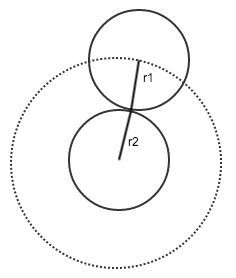
\includegraphics[width=2in]{quarters.png}
  \caption{}
  \label{fig:quarters}
\end{figure}

The center of the moving circle travels along the dotted circle. That circle has circumference $2\pi(r_1+r_2)$. Computing linear displacement along this longer path effectively cancels the ``rotational advantage'' in the model above, so you can compute the number of rotations directly: $2\pi(r_1+r_2) / 2{\pi}r_1 = (r_1 + r_2) / r_1 = 1 + r_2/r_1$.

The degenerate cases are interesting and good to check.  If $r_2$ is zero, you get $1$ which makes sense, since you are just spinning the top circle around a point.  If $r_1$ is zero, things are hopeless - you get nowhere spinning a zero-radius wheel. If, as in the round-the-world example, $r1$ is much smaller than $r_2$, the ``$+1$'' is negligible.




\end{document}